% \documentclass[fleqn,10pt]{wlscirep}
% fleqn : left alignment of equation

\documentclass[fleqn, 10pt]{wlscirep}
\usepackage[utf8]{inputenc}
\usepackage{amsmath}
\usepackage{amsbsy}
\usepackage{xcolor}
\usepackage[T1]{fontenc}
\usepackage{soul} % 여러 라인에 걸친 밑줄을 사용하기 위한 패키지

% \usepackage[style=authoryear,backend=biber]{biblatex}
\DeclareMathOperator*{\argmin}{arg\,min} % Jan Hlavacek

%from here, code for line numbers
\usepackage{lineno}
\linenumbers

\makeatletter
\patchcmd\@maketitle{%
        {%
        \noindent
        \colorbox{color2}{%
            \parbox{\dimexpr\linewidth-2\fboxsep\relax}{%
            \sffamily\small\textbf\\\theabstract
            }%
        }%
        }%
    }{%
        \nolinenumbers{%
        \noindent
        \colorbox{color2}{%
            \parbox{\dimexpr\linewidth-2\fboxsep\relax}{%
            \internallinenumbers \sffamily\small\theabstract
            }%
        }%
        }%
    }
    {\wlog{true}}{\wlog{false}}
    
\makeatother
%end of code for line numbers

\title{Backward Cumulative Channel Sum-Based Spectral Processing for Radionuclide Identification in Plastic Scintillation Detectors}
% \linenumbers
\author[1]{Ji-Yong So}
\author[2]{Byoungil Jeon}
\author[1,*]{Myungkook Moon}
\affil[1]{Korea Atomic Energy Research Institute, Neutron Science Division, Daejeon, 34057, Korea}
\affil[2]{Korea Atomic Energy Research Institute, Applied Artificial Intelligence Section, Daejeon, 34057, Korea}

\affil[*]{moonmk@kaeri.re.kr}

% \affil[+]{These authors equally contributed to this work}

\keywords{radiation portal monitor, radionuclide identification}

\begin{abstract}

Plastic scintillation detectors are widely used in radiation monitoring systems because of their high detection efficiency, fast response, and robust operation. However, reliable radionuclide discrimination remains difficult because plastic scintillators exhibit poor energy resolution, broad Compton-dominated spectral distributions, and strong sensitivity to background variation in practical measurement environments.

In this study, we propose a backward cumulative channel sum (BCCS)-based spectral processing framework for improving radionuclide discrimination using large plastic scintillation detectors. The proposed method preserves the global spectral characteristics of plastic scintillator responses while reducing local statistical fluctuations through cumulative transformation. After BCCS preprocessing, subtraction-based and normalization-based background compensation methods were applied, and the resulting spectra were analyzed using a non-negative least squares (NNLS)-based linear unfolding framework.

The method was evaluated using Am-241, Cs-137, and Co-60 under both single-source and mixed-source conditions. The results showed that the BCCS transformation provides a more stable spectral representation than the raw spectrum, enhances radionuclide-dependent spectral differences, and enables practical decomposition of mixed-source spectra. The subtraction-based method preserves net signal-scale information, whereas the normalization-based method provides improved flexibility under varying acquisition conditions.

Overall, the proposed BCCS-based framework provides a practical and physically meaningful approach for extracting radionuclide-specific information from low-resolution plastic scintillator spectra under low-count, mixed-source, and background-varying conditions, and is expected to be useful for real-time radiation monitoring and container inspection applications.

\end{abstract} 

\begin{document}

\flushbottom
\maketitle

\thispagestyle{empty}


\section*{Introduction}

Plastic scintillation detectors are widely used in radiation portal monitors (RPMs) and other
field-deployable radiation monitoring systems because of their high detection efficiency, fast response, and robust operation\cite{Sicilliano2005Comparision, Bertrand2014Current,Ely2006TheUse,Hevener2013EWindow}. However, reliable radionuclide identification using plastic scintillators remains challenging because of their inherently poor energy resolution and broad spectral distributions dominated by Compton scattering\cite{Hevener2013EWindow, Lee2020Radioisotope, Paff2017Spectral,Runkle2006Analysis}. 

This difficulty becomes more significant in practical RPM environments. During container inspection, the container itself and the cargo inside it can partially attenuate radiation and alter the measured background spectrum. As a result, background intensity and spectral shape may vary depending on the inspected object, making radionuclide discrimination based only on gross counts unreliable\cite{Lee2020Radioisotope, Paff2017Spectral,Runkle2006Analysis,Kim2019InvMat}. Under such conditions, more effective use of spectral shape information is required.

Under identical background conditions, the spectral response of a given radionuclide preserves its overall shape while its amplitude scales with source intensity. Although discrete counting statistics introduce small fluctuations, the characteristic spectral pattern remains stable. This property provides the basis for constructing radionuclide-specific reference spectra and for interpreting mixed-source measurements as linear combinations of these reference patterns.

Several approaches have been proposed to improve radionuclide identification in low-resolution detectors, including spectral windowing\cite{Ely2006TheUse,Hevener2013EWindow}, statistical feature extraction methods based on principal component analysis\cite{Runkle2006Analysis,Kim2019InvMat}, 
%\begin{comment}unfolding-based methods,\end{comment} 
and machine-learning-based classification\cite{Kim2019ANN, Lee2023Radionuclide,Jeon2021CompML}. However, their practical applicability may be limited in real RPM environments, where a container truck passes the detector within a short time and a localized radioactive source contributes significantly to the measured spectrum only during a brief interval when it is close to the detector. Under such conditions, the measured signal is often affected by limited counting statistics, variable background, and mixed-source characteristics.

In this study, we propose a backward cumulative channel sum (BCCS)-based spectral processing method for plastic scintillation detectors. The proposed method uses the full spectral information while reducing statistical fluctuations through cumulative transformation, thereby preserving the global spectral shape and enhancing subtle differences between radionuclides. Once radionuclide-specific reference spectra are transformed into the BCCS domain, mixtures of multiple radionuclides can be analyzed using a least-squares-based decomposition framework to estimate their relative
contributions.

% To evaluate the characteristics of the proposed method, three representative radionuclides—Am-241, Cs-137, and Co-60—were selected in this study. These radionuclides have relatively long half-lives and distinct energy distributions, making them suitable for assessing the performance of the BCCS-based approach under both single-source and mixed-source conditions.

To evaluate the proposed BCCS-based approach, three representative radionuclides—Am-241, Cs-137, and Co-60—were selected as test cases. These radionuclides have relatively long half-lives and exhibit distinct spectral characteristics in plastic scintillation detectors and thus provide a practical basis for assessing the method under both single-source and mixed-source conditions.

\section*{Methods}
\subsection*{Experimental Setup}

All measurements were performed using the same plastic scintillation detector system under identical detector geometry conditions. The detector consisted of a plastic scintillator
with dimensions of 30 cm $\times$ 180 cm $\times$ 5 cm, coupled to a photomultiplier tube (PMT). The
detector size and measurement configuration were kept unchanged throughout the experiments in order to ensure consistent comparison among single-source, mixed-source, and background measurements.

Background measurements were acquired in the absence of any radioactive source. The background count rate depended slightly on the lower level discriminator (LLD) setting. Under the measurement condition used in this study, where the LLD was set to include the energy region relevant to Am-241 detection, the background count rate was approximately 10,000 cps per detector. This background condition was used as the reference for both subtraction-based and normalization-based spectral processing.

% Three representative radionuclides, Am-241, Cs-137, and Co-60, were selected for evaluation of the proposed method. These radionuclides were chosen because they have relatively long half-lives and distinct representative energy regions, allowing systematic comparison of their spectral characteristics. In addition to single-source measurements, mixed-source conditions were also prepared to evaluate decomposition performance.


Three representative radionuclides, Am-241, Cs-137, and Co-60, were selected for evaluation of the proposed method. The corresponding source activities were 90 $\mu\text{Ci}$, 16 $\mu\text{Ci}$, and 9 $\mu\text{Ci}$, respectively. Single-source measurements were used to construct radionuclide-specific reference spectra, and mixed-source configurations were additionally prepared to evaluate decomposition performance.

In addition to the controlled reference and mixed-source measurements described above, a separate real-time validation test was conducted under container-transfer conditions to examine the practical applicability of the proposed framework.


\subsection*{Spectral Channel Configuration}

In scintillation detector systems, spectral data are commonly acquired using 256, 512, or 1024 channels, whereas high-resolution semiconductor detectors such as HPGe often use much finer channel configurations, such as 4k or 8k channels. However, for plastic scintillation detectors, increasing the number of channels does not necessarily improve radionuclide discrimination because of the intrinsically low energy resolution of the detector response.

In this study, the spectral data were analyzed using 256 channels. The reason for this choice is that increasing the number of channels reduces the counts per channel and degrades counting statistics, while providing little additional discriminative information for plastic scintillator spectra. Therefore, the use of 256 channels provides a practical balance between spectral representation and statistical reliability for plastic scintillator-based measurements. This choice is particularly appropriate for plastic scintillation detectors, in which statistical
fluctuations are more influential than fine spectral resolution.


\subsection*{Spectral Preprocessing: Backward Cumulative Channel Sum (BCCS)}

The backward cumulative channel sum (BCCS) is defined as a cumulative transformation of the pulse-height spectrum. Let $\mathbf{C} = [C_1,\,C_2,\ldots,\,C_N]$ denote the raw pulse-height spectrum, where $C_i$ is the count in channel $i$. The BCCS spectrum is given by

\begin{equation}
B_i = \sum_{j=i}^N C_j. \label{eq:BCCS}
\end{equation}

This transformation produces a monotonically decreasing representation of the spectrum, reducing statistical fluctuations while preserving the global spectral shape. Because plastic scintillator spectra are dominated by broad Compton-related distributions rather than sharp photopeaks, preservation of the overall spectral shape is more important than retaining fine channel-by-channel variations.


During method development, both forward and backward cumulative summation schemes were examined. The forward cumulative sum is defined as

$$
F_i = \sum_{j=1}^i C_j. \label{eq_FCCS}
$$

In the forward cumulative representation, the cumulative values are constructed from the lowest channels upward. Because the spectral features relevant for radionuclide discrimination in plastic scintillators are primarily located in the low- to medium-channel region, the forward scheme provides limited noise suppression in these critical channels. As a result, statistical fluctuations in the most informative part of the spectrum remain largely unmitigated.
In contrast, the backward cumulative representation integrates counts from each channel toward the high-channel end of the spectrum. This leads to substantial averaging even in the low- and medium-channel region, where most of the physically meaningful spectral differences reside. Consequently, the backward scheme more effectively reduces statistical fluctuations in the most relevant part of the spectrum while preserving the global spectral trend.
For these reasons, the backward cumulative channel sum (BCCS) was adopted in this study as the primary spectral transformation method.


For each measurement condition, repeated acquisitions were performed more than 10 times under identical experimental settings. Because the run-to-run variation in spectral shape and in the resulting BCCS trend was negligible, a single representative spectrum is presented in the figures for clarity.

% Unlike the conventional forward cumulative spectrum that sums from the first channel upward, the BCCS accumulates counts from channel 
% $i$ to the end of the spectrum. This produces a smooth, monotonically decreasing cumulative profile that suppresses statistical fluctuations in the high-channel region while preserving the global spectral structure. Because this transform enhances separability under low-count conditions, it serves as the primary preprocessing step for all subsequent analyses.


\subsection*{Background Compensation Techniques}

After BCCS preprocessing, background compensation was applied to reduce the influence of ambient radiation and system background on the transformed spectra. In practical RPM environments, both the intensity and spectral shape of the background may vary depending on container structure, cargo composition, and measurement conditions. Therefore, appropriate background compensation is essential prior to radionuclide spectral decomposition.

Two background compensation techniques were considered in this study. The first was a subtraction-based method, defined as 

\begin{equation}
S^M_i =  B^M_i - B_i^{\textrm{bkg}}. \label{eq:DS}
\end{equation}

where $B_i^M$ and $B_i^\text{bkg}$ denote BCCS spectra of the measured signal and background, respectively. This approach preserves the net count scale of the source contribution and is suitable when absolute signal magnitude is relevant for interpretation, although it may also amplify statistical fluctuations when the count level is low.

The second was a normalization-based method, defined as 

\begin{equation}
R^M_i = \left(\dfrac{B^M_i}{B^{\textrm{bkg}}_i}\right) -1.\label{eq:NB}
\end{equation}

This formulation represents the relative deviation of the measured spectrum from the background. The subtraction of unity ensures that 
$R_i^M = 0$ corresponds to pure background, providing a convenient baseline for comparison. Because the ratio removes the common scaling factor between the measured and background spectra, it is largely independent of acquisition time and overall count scale. This property is particularly useful in real-time inspection systems, where the effective measurement time may vary as a container truck passes the detector.


In both compensation schemes, the spectral data can also be converted into count-rate form by dividing the measured counts by the acquisition time. In this case, the spectral values are no longer restricted to integers and may take fractional values. However, this does not affect the BCCS procedure, because the cumulative summation can be applied equally to integer and non-integer values. Therefore, the proposed method remains applicable even when the measurement time varies. This property is particularly important in practical RPM environments, where container trucks do not always pass the detector at a constant speed.

Both compensation methods were applied in the BCCS domain, and their performances were compared in terms of spectral contrast, stability, and robustness in subsequent decomposition analysis.

\subsection*{Radionuclide Activity Estimation via Linear Spectral Unfolding}

Following BCCS preprocessing and background compensation, the processed spectrum was analyzed using a linear spectral unfolding framework. Under fixed detector geometry and comparable background conditions, the processed spectrum can be approximated as a linear combination of radionuclide-specific reference spectra.

For the subtraction-based representation, the processed spectrum is expressed as
\begin{equation}
S_i^{M} = \sum_{X} \alpha_X S_i^{X},
\label{eqn:subtraction_unfolding}
\end{equation}
where $\alpha_X$ denotes the relative contribution of radionuclide $X$.

For the normalization-based representation, the situation is slightly different because the normalized spectrum depends explicitly on the background spectrum used for normalization. If the background spectra of the measured and reference data are sufficiently similar under the same measurement conditions, i.e.,
\begin{equation}
B_i^{M,\mathrm{bkg}} \approx B_i^{X,\mathrm{bkg}},
\label{eqn:bkg_similarity}
\end{equation}
the normalized processed spectrum can be approximated as
\begin{equation}
R_i^{M} \approx \sum_{X} \alpha_X R_i^{X}.
\label{eqn:ratio_unfolding}
\end{equation}

In both cases, the radionuclide contributions were estimated by solving a non-negative least squares (NNLS) problem:
\begin{equation}
\{\alpha_X\}
=
\argmin_{\alpha_X \ge 0}
\sum_{i=1}^{N}
\left(
I_i^{M} - \sum_{X}\alpha_X I_i^{X}
\right)^2,
\label{eqn:nnls}
\end{equation}

\noindent where $I_i^{M}$ denotes the processed spectrum of the measured data, $I_i^{X}$ denotes the processed reference spectrum for radionuclide $X$, and $I_i$ represents either the subtraction-based or normalization-based spectral form depending on the compensation method used. The non-negativity constraint ensures physically meaningful solutions by preventing negative radionuclide contributions.

Because meaningful source-dependent information in plastic scintillator spectra is concentrated mainly in the low- and medium-channel region, the unfolding analysis was performed over a restricted channel range. This reduces the influence of high-channel statistical fluctuations while preserving the spectral information relevant for radionuclide discrimination.

The resulting coefficients do not represent absolute radionuclide activities in becquerels, because the moving measurement geometry does not permit direct activity quantification. Instead, they are interpreted as reference-based indicators of relative contribution and relative signal level for each radionuclide.



\section*{Results}

%Up to three levels of \textbf{subheading} are permitted. Subheadings should not be numbered.

\subsection*{BCCS Transformation of Reference Radionuclide Spectra}

Figure \ref{fig:bkgref}(a) shows the raw spectra of background radiation and three reference radionuclides, Am-241, Cs-137, and Co-60, measured using a large-volume plastic scintillation detector. As expected for plastic scintillators, the spectra are dominated by broad Compton continua rather than sharp photopeaks, and most counts are concentrated in the low-channel region. Under these conditions, direct visual discrimination based on the raw spectra is limited, particularly when the net source contribution is weak.

After application of the BCCS transformation, the spectra are converted into smooth and monotonically decreasing profiles, as shown in Figure \ref{fig:bkgref}(b). This transformation suppresses channel-to-channel statistical fluctuations while preserving the overall spectral tendency of each radionuclide. As a result, the BCCS representation provides a more stable basis for qualitative comparison among radionuclides than the raw spectral form.

Figures \ref{fig:bkgref}(c) and \ref{fig:bkgref}(d) show the background-subtracted and background-normalized BCCS spectra, respectively. In the subtraction-based representation, the net source contribution is preserved on an absolute net signal-scale, which is advantageous when relative signal magnitude is important. In the normalization-based representation, the spectra are expressed as relative deviations from the background, providing improved comparability under varying measurement conditions. In both forms, radionuclide-dependent spectral differences are more clearly distinguished than in the raw spectra.

It should be noted that the small Am-241 values observed in the high-channel region do not have physical significance. They originate from statistical fluctuations in the original low-count data and were retained without additional artificial suppression.

\subsection*{Comparison of Background Compensation Methods for Mixed-Source Spectra}

Figure \ref{fig:mixedbccs} presents the BCCS spectra for nine mixed-source configurations after applying the two background compensation methods. In Figure \ref{fig:mixedbccs}(a), the subtraction-based representation preserves absolute net signal-scale differences among the mixed-source cases, allowing comparison of both spectral shape and relative signal magnitude. This form is advantageous when the net source contribution itself is of interest in the subsequent fitting procedure.

In contrast, Figure \ref{fig:mixedbccs}(b) shows that the normalization-based representation expresses the spectra as relative deviations from the background. As a result, differences among mixed-source conditions are more directly comparable even when the overall count level varies. This property is particularly useful in practical RPM situations, where the effective acquisition time and total count rate may change depending on source position or container motion.

The two compensation methods therefore provide complementary advantages. The subtraction-based form retains absolute net signal information, whereas the normalization-based form provides a more flexible representation under varying measurement conditions. In both cases, the BCCS-processed spectra preserve sufficient radionuclide-dependent structure for subsequent decomposition analysis.


\subsection*{Linear spectral unfolding of mixed-source measurements}

The unfolding results for the mixed-source spectra are presented in Figures \ref{fig:fi_fitbgsub} and \ref{fig:fi_fitbgrto}. In both cases, the processed BCCS spectra are well reproduced by the fitted combinations of reference radionuclide spectra, indicating that the mixed-source response can be reasonably described within the proposed reference-based linear unfolding framework.

Figure \ref{fig:fi_fitbgsub} shows the results obtained using subtraction-based BCCS processing. The measured spectra are decomposed into Am-241, Cs-137, and Co-60 components with non-negative coefficients, and the fitted curves follow the overall spectral trends of the mixed-source data closely. It should be noted, however, that small nonzero contributions may also be assigned to radionuclides that were not intentionally included in a given source configuration. Such residual components are attributable to limited separability among low-resolution plastic scintillator spectra and to statistical fluctuations in the measured data, rather than to unambiguous evidence for the presence of that radionuclide. In the mixed-source cases examined here, the dominant coefficients nevertheless correspond to the radionuclides actually present, while the residual components remain comparatively small.

Figure \ref{fig:fi_fitbgrto} shows the corresponding results obtained using normalization-based BCCS processing. The decomposition remains stable in the normalized representation, while reducing sensitivity to variations in overall count scale and effective acquisition time. As in the subtraction-based case, small residual contributions can appear for radionuclides not present in the source configuration, but the dominant coefficients remain consistent with the actual source composition. This property is particularly useful in practical RPM conditions, where the duration of source exposure may vary owing to non-uniform container motion.

In both representations, the unfolding analysis was restricted to the low- and medium-channel region, where the source-dependent spectral information is concentrated in plastic scintillator spectra. This reduces the influence of high-channel statistical fluctuations while preserving the spectral features relevant for radionuclide discrimination.

Overall, the results show that BCCS preprocessing, combined with background compensation and NNLS-based unfolding, provides a practical framework for decomposing mixed-source plastic scintillator spectra under low-resolution and variable-background conditions.


\subsection*{Relative Signal Level as a Function of Source-to-Detector Distance}

Figure \ref{fig:fi_fitcontrib} summarizes the estimated coefficients as a function of source-to-detector distance for the three reference radionuclides. In both the subtraction-based and normalization-based analyses, the coefficient associated with the corresponding radionuclide decreases monotonically as the distance increases. This trend is consistent with the reduction in detector response caused by geometric attenuation and the corresponding decrease in net source contribution.

At sufficiently large distance, the estimated coefficient approaches the level obtained when the corresponding radionuclide is absent. This behavior reflects the practical limit at which radionuclide-specific information becomes difficult to distinguish from background-related variation and residual fitting components. The horizontal dashed lines therefore provide a useful reference level for practical discrimination, indicating the range below which the inferred contribution is no longer clearly distinguishable from the no-source case.

As discussed above, the coefficients obtained from the unfolding procedure should not be interpreted as absolute radionuclide activities in becquerels. Instead, they represent reference-based indicators of relative signal level and relative contribution under the given measurement conditions. In this sense, the results in Figure \ref{fig:fi_fitcontrib} demonstrate that the proposed framework provides physically consistent trends with changing measurement geometry, while retaining practical utility for radionuclide identification.

\section*{Discussion}


The results demonstrate that the proposed BCCS-based framework provides a stable and practical spectral representation for radionuclide analysis using large plastic scintillation detectors. Because plastic scintillators produce broad Compton-dominated spectra rather than sharp photopeaks, radionuclide-dependent information is distributed over the overall spectral shape rather than concentrated in narrow spectral features. In this context, the BCCS transformation is effective because it suppresses local statistical fluctuations while preserving the global spectral trend relevant for radionuclide discrimination.

An important feature of the proposed framework is that it makes use of spectral shape information rather than relying only on gross count variation. In practical RPM environments, both the background level and the measured spectral distribution can vary owing to container structure, cargo composition, and changing measurement geometry. Under such conditions, radionuclide identification based only on total count rate can be unreliable. The BCCS representation provides a more stable basis for comparing spectra and for identifying source-dependent deviations from the background, even when the raw spectral differences are not visually distinct.

The comparison between subtraction-based and normalization-based background compensation further clarifies the practical utility of the method. The subtraction-based representation preserves the absolute scale of the net source contribution and is therefore advantageous when relative signal magnitude is important in reference-based fitting. In contrast, the normalization-based representation expresses the spectrum as a relative deviation from the background and is therefore more flexible under varying acquisition conditions. In the present study, both approaches produced stable unfolding results, suggesting that they should be regarded as complementary compensation strategies rather than competing alternatives.

The unfolding results also show that mixed-source spectra can be analyzed within a reference-based linear decomposition framework, provided that detector geometry and background conditions remain sufficiently comparable. Although small residual contributions may appear for radionuclides not actually present in a given source configuration, these components remain much smaller than the dominant coefficients associated with the true sources. This behavior reflects the limited separability of low-resolution plastic scintillator spectra and the influence of statistical fluctuations, rather than direct evidence of false radionuclide presence. From a practical point of view, this suggests that the coefficients should be interpreted in a relative sense, together with appropriate reference or threshold levels, rather than through strict zero/nonzero criteria.

The distance-dependent trends shown in Figure \ref{fig:fi_fitcontrib} further support this interpretation. As the source-to-detector distance increases, the estimated coefficient decreases monotonically toward the level observed in the absence of the corresponding radionuclide. This behavior is physically consistent with the reduction in detector response caused by geometric attenuation and decreasing net source contribution. The resulting coefficients should therefore be understood not as absolute activities in becquerels, but as reference-based indicators of relative signal level under the given measurement conditions.

The present validation was performed using three representative radionuclides, Am-241, Cs-137, and Co-60, which were selected as practical test cases with distinct spectral characteristics. The proposed framework, however, is not restricted to these radionuclides. If additional reference spectra are acquired under comparable conditions, the same BCCS-based processing and unfolding procedure can be extended to a broader radionuclide set. In this sense, the present study should be regarded as a proof-of-concept validation of the method rather than as a limitation of its applicability.

Several practical limitations should also be noted. The method depends on the availability of representative reference spectra, and its performance may degrade if detector response or background conditions differ substantially from those used to construct the reference set. In addition, environmental effects such as gain drift can alter the measured spectral distribution. In practical operation, these effects may be mitigated by updating background and reference data under current measurement conditions. Despite these limitations, the results indicate that the proposed framework provides a physically well-motivated and practically useful approach for extracting radionuclide-specific information from low-resolution plastic scintillator spectra without requiring high-resolution detector hardware or data-intensive learning procedures.

Additional practical validation was also performed under container-transfer conditions using Am-241, Cs-137, and Co-60 sources attached to containers. In this test, the spectrum measured during the interval between successive containers was used as the operational background, and radionuclide identification was performed using the subtraction-based BCCS framework. Under the tested conditions, the source configuration was correctly identified in 99 of 100 trials. Although this validation was limited to the radionuclides and operating conditions examined here, it provides additional evidence for the practical applicability of the proposed approach in realistic container-screening scenarios; a detailed account of this validation study will be reported elsewhere \cite{Unpublished1}.



\section*{Conclusion}

In this study, a BCCS-based spectral processing framework was proposed for radionuclide discrimination using large plastic scintillation detectors under practical RPM-like conditions. The method was designed to preserve the global spectral characteristics of plastic scintillator responses while reducing local statistical fluctuations through cumulative transformation.

The results showed that the BCCS representation provides a stable basis for comparing radionuclide-dependent spectral patterns and for decomposing mixed-source spectra in combination with background compensation and NNLS-based unfolding. The subtraction-based representation preserves net signal-scale information, whereas the normalization-based representation provides improved flexibility under varying acquisition conditions.

The unfolding coefficients obtained in this framework should be interpreted as reference-based indicators of relative contribution and relative signal level, rather than as absolute radionuclide activities. Within this interpretation, the proposed method provides a practical and physically meaningful approach for extracting radionuclide-specific information from low-resolution plastic scintillator spectra.

Although the present study focused on three representative radionuclides, the framework can be extended to additional radionuclides when appropriate reference spectra are available. The proposed approach is therefore expected to be useful for real-time radiation monitoring and container inspection applications.


\section*{Acknowledgements}

This research was supported by the Ministry of Oceans and Fisheries, Korea, through the Korea Institute of Marine Science \& Technology Promotion (KIMST) under Project No. 20200611. The authors acknowledge the use of ChatGPT (OpenAI) for language refinement and editorial assistance during the preparation of this manuscript. All scientific content, interpretations, and conclusions presented herein were solely developed and validated by the authors.

\section*{Author contributions statement}
M. Moon conceived the study and performed the experiments. J. So developed the analysis software and performed signal processing. B. Jeon synthesized the test datasets and supported evaluation. All authors contributed to writing and reviewing the manuscript.


\bibliography{biblio}


\begin{figure}[ht]
\centering
% 
\includegraphics[width=\linewidth]{figure/fig01_bkgref.pdf}
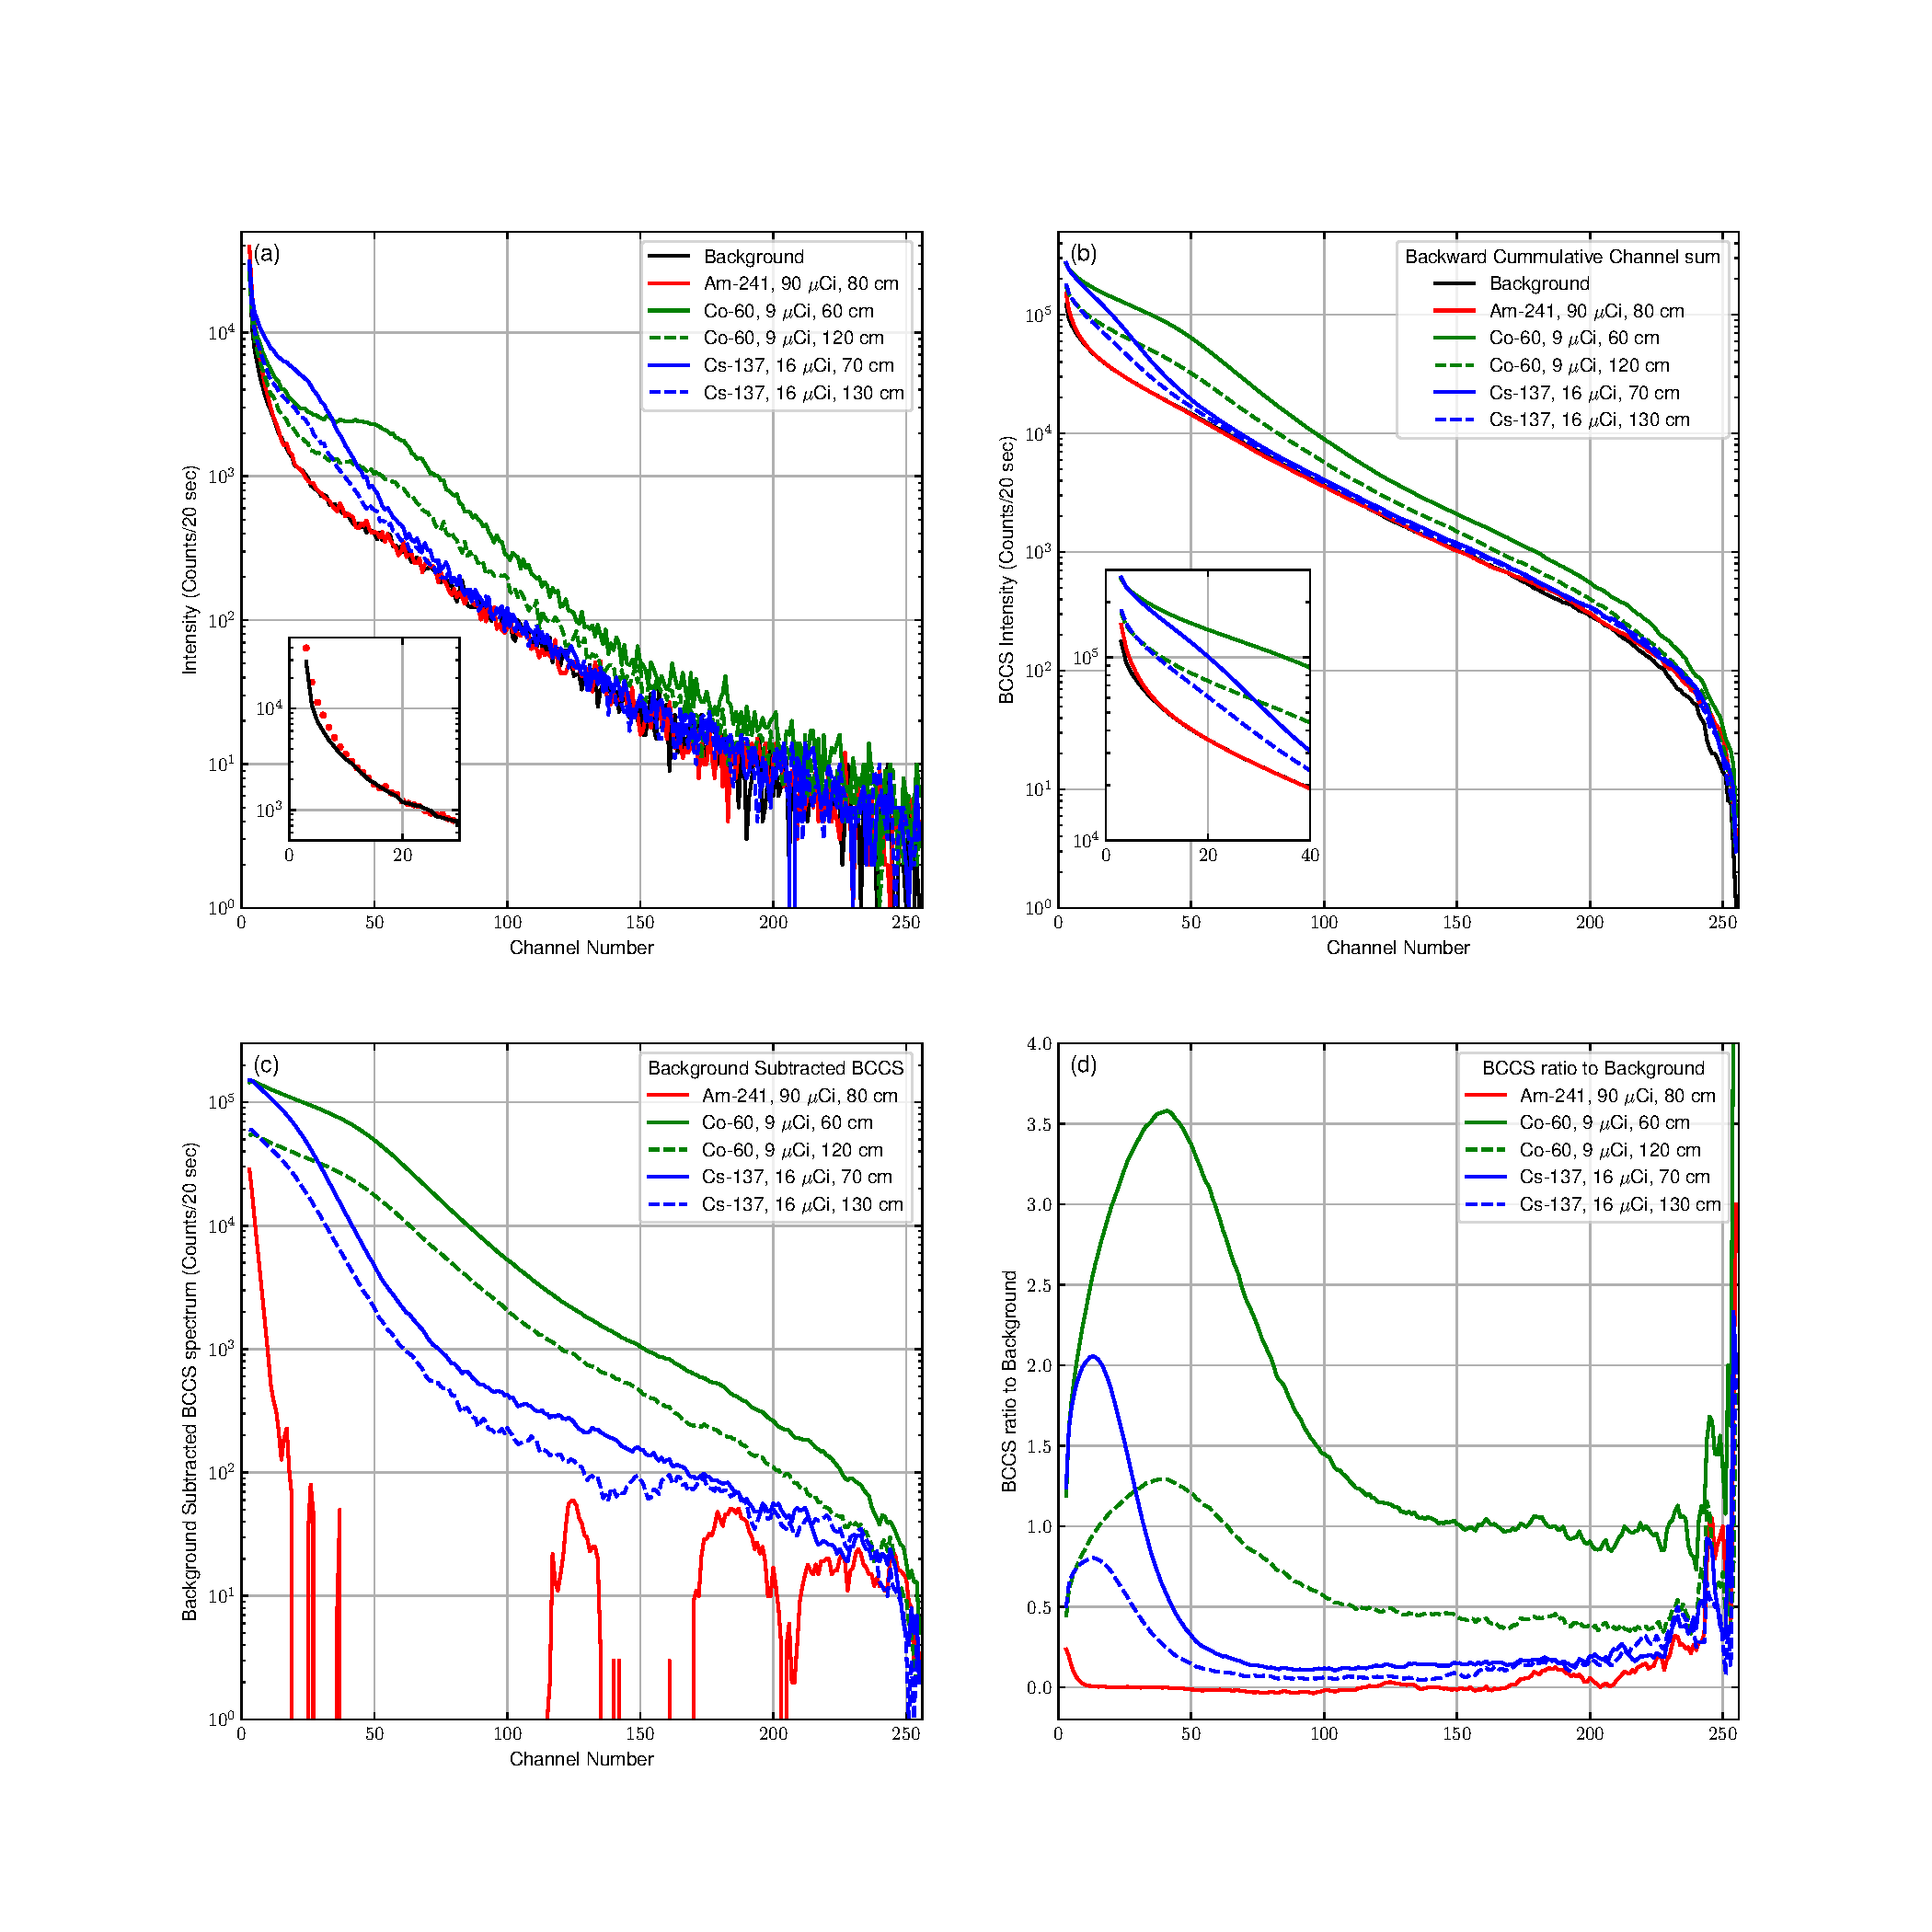
\includegraphics[width=\linewidth]{newfigures/figure1.pdf}
\caption{Spectral comparison of the background and reference radionuclides before and after BCCS processing. (a) Raw spectra of the background, Am-241, Cs-137, and Co-60 measured with the plastic scintillation detector. (b) Corresponding BCCS-transformed spectra. (c) Background-subtracted BCCS spectra. (d) Background-normalized BCCS spectra. The BCCS transformation produces smooth, monotonically decreasing profiles while preserving radionuclide-dependent spectral differences. Small Am-241 values in the high-channel region originate from statistical fluctuations in the measured low-count data and do not represent physically meaningful spectral structure.}

\label{fig:bkgref}
\end{figure}

\newpage 

\begin{figure}[ht]
\centering
% 
\includegraphics[width=\linewidth]{figure/fig04_CSBS.pdf}
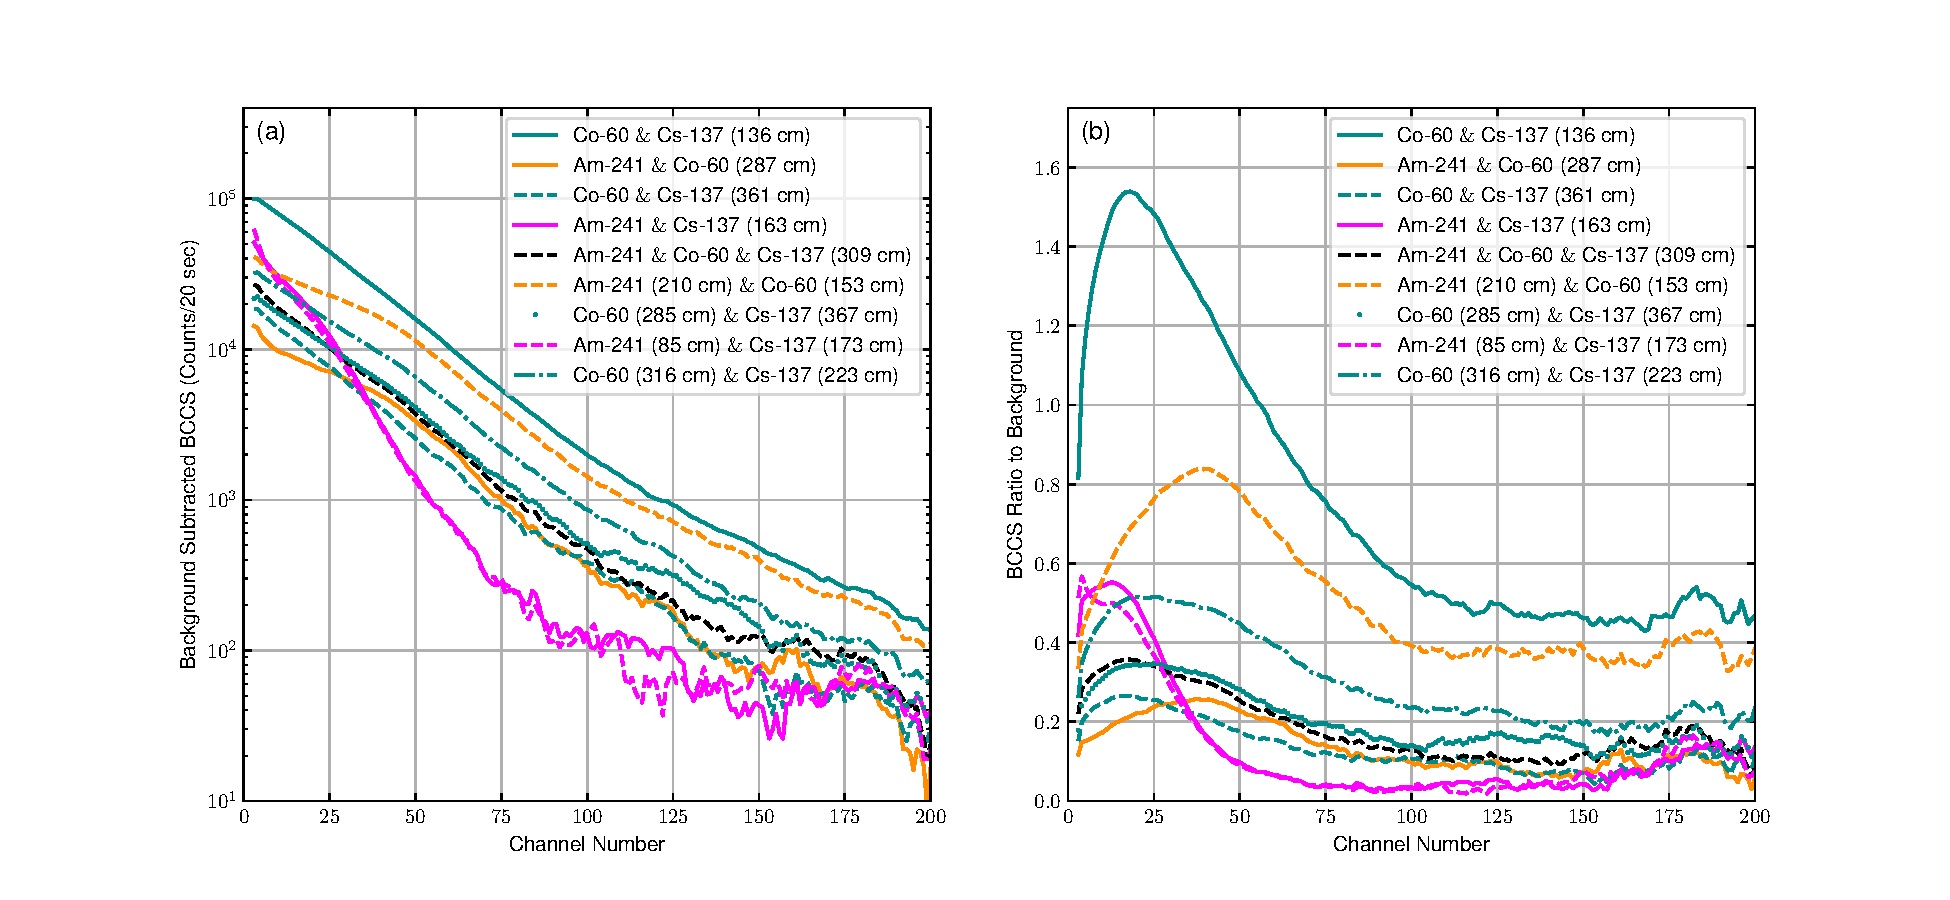
\includegraphics[width=\linewidth]{newfigures/figure2.pdf}
\caption{Comparison of BCCS spectra for nine mixed-source configurations using two background compensation methods. (a) Background-subtracted BCCS spectra. (b) Background-normalized BCCS spectra. The subtraction-based representation preserves absolute net signal-scale differences among the mixed-source cases, whereas the normalization-based representation expresses the spectra as relative deviations from the background and provides improved comparability under varying acquisition conditions.}
\label{fig:mixedbccs}
\end{figure}

\newpage


\begin{figure}[ht]
\centering

\includegraphics[width=\linewidth]{newfigures/fit_BGSub.pdf}
\caption{Linear spectral unfolding results for mixed-source spectra using subtraction-based BCCS processing. The processed BCCS spectra (solid lines) are fitted by linear combinations of the reference radionuclide spectra (dashed lines). The results show that the mixed-source spectra can be decomposed into Am-241, Cs-137, and Co-60 components with non-negative coefficients. Small residual contributions may also appear for radionuclides not intentionally included in a given source configuration because of limited separability in low-resolution plastic scintillator spectra and statistical fluctuations.}
\label{fig:fi_fitbgsub}
\end{figure}

\begin{figure}[ht]
\centering

\includegraphics[width=\linewidth]{newfigures/fit_BGRto.pdf}
\caption{Linear spectral unfolding results for mixed-source spectra using normalization-based BCCS processing. The normalized processed spectra are fitted by linear combinations of the normalized reference spectra. The normalization-based representation provides stable decomposition while reducing sensitivity to variations in overall count scale and effective acquisition time. As in the subtraction-based case, small residual contributions may appear for radionuclides not present in a given source configuration.}
\label{fig:fi_fitbgrto}
\end{figure}

\begin{figure}[ht]
\centering
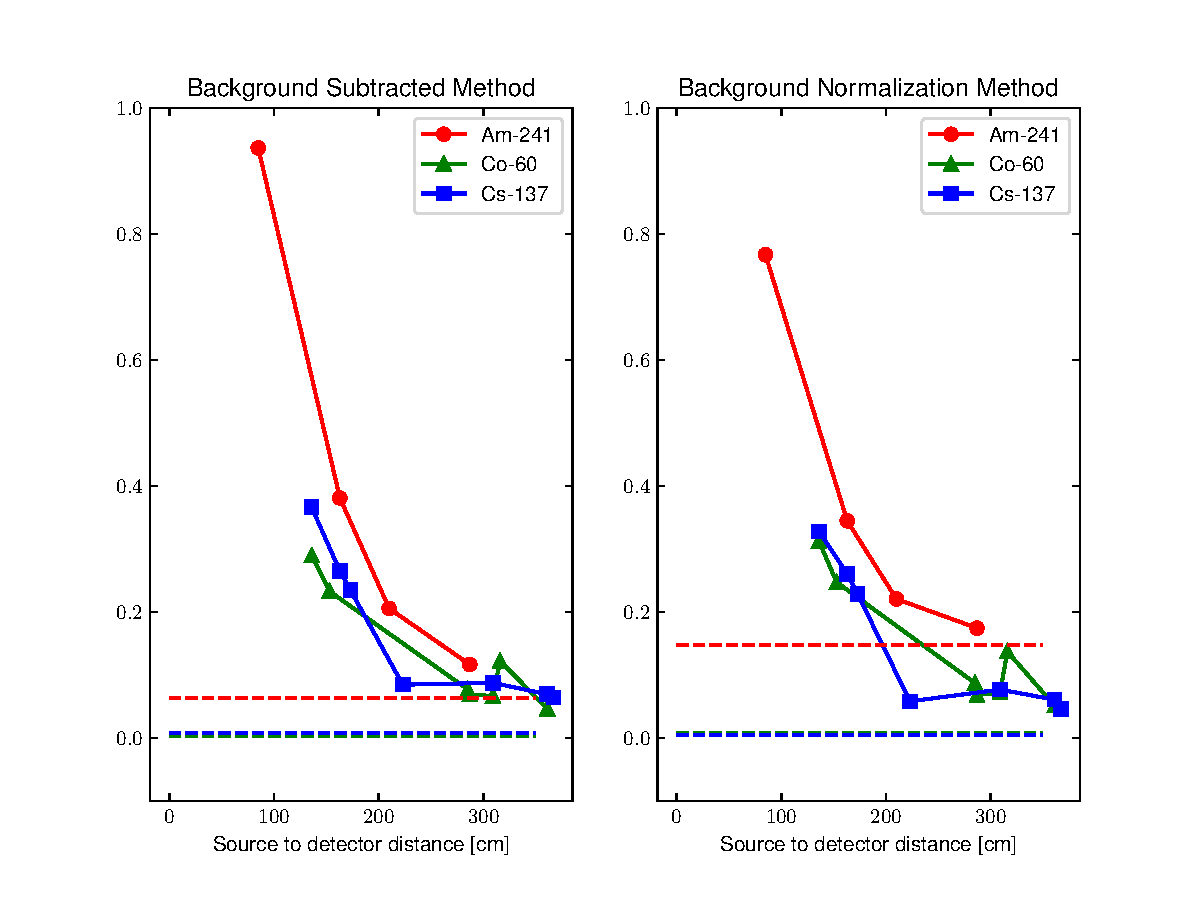
\includegraphics[width=\linewidth]{newfigures/fit_contributions.pdf}
\caption{Variation of the estimated radionuclide coefficients with source-to-detector distance for the subtraction-based and normalization-based methods. The coefficients obtained from spectral unfolding represent reference-based relative signal levels rather than absolute activities. The horizontal dashed lines indicate, for each radionuclide, the mean coefficient obtained from NNLS fitting of spectra in which that radionuclide was absent, and serve as practical reference levels for discrimination. As the distance increases, the estimated coefficient decreases because of geometric attenuation and the corresponding reduction in net detector response. The plotted results are representative; each condition was repeated more than 10 times under identical settings, and the overall trend was reproducible.}
\label{fig:fi_fitcontrib}
\end{figure}

\end{document}